\documentclass[b5paper,papersize,dvipdfmx,fleqn]{jsarticle}
\usepackage{/Users/yamasakishun/Desktop/ymskarticle}
\usepackage{here}

\begin{document}
\title{Essay}
\author{05-201564 Shun Yamasaki}
\date{\today}
\maketitle

\section{Abstract}
Solving linear equations is a very important problem in many situations as we know \cite{Harrow2009}. A inear equations is
\begin{eqnarray}
  A\vec{x} = \vec{b}.
\end{eqnarray}

In this paper, we assume that we do not need to know $\vec{x}$ itself, but we want to find a value related to $\vec{x}$ such as $\vec{x}^\dagger M \vec{x}$, where $M$ is a certain matrix. Consider the case where $A$ is a matrix of $N\times N$ with up to $s$ non-zero components per row and the condition number \footnote{condition number is an upper bound on the uncertainty of the solution of a linear equation and is defined as the maximum ratio of the relative error of $x$ divided by the relative error of $b$. It is defined as the maximum ratio of the relative error of $x$ divided by the relative error of $b$.} is $\kappa $, the fastest known classical algorithm can calculate $\vec{x}, \vec{x}^\dagger M\vec{x}$ in a time scale of $N\sqrt{\kappa }$.
On the other hand, in the quantum algorithm presented here, when the state $\ket{b}$ corresponding to $\vec{b}$ is available, the computational steps to find $\ket{x}$ can be computed on a polynomial time scale of $\log(N)$ and $\kappa $. This is an exponential speedup compared to classical computers.

\section{Introduction}
% \subsection{Quantum Computer}

A quantum computer is a device that uses quantum mechanics to perform calculations, including calculations that are not possible with currently known algorithms from classical computers. For certain problems, such as Shor's algorithm, a quantum computer can perform calculations much faster than a classical computer. In this paper, we will consider the characteristics of the solution of a linear system of linear equations.

%\subsection{Linear Equation}

Linear equations have applications in almost every field of science, technology, and engineering, and are very important\cite{Harrow2009}. On a classical computer, it generally takes at least $N$ orders of time to solve a $N$-order linear equation.

%\subsection{Overview}

In this paper, we use the same equations as in Abstract;
\begin{eqnarray}
  A\vec{x} = \vec{b}.
\end{eqnarray}
If $A$ is a $N\times N$ matrix with up to $s$ non-zero components per row, and the condition number is $\kappa $, then it shows that it takes a polynomial time scale of $\log(N),\kappa $ to compute the values associated with the solution $\ket{x}$ to any precision. This is an exponential speedup compared to a classical computer. Also, in typical cases, accuracy is not often required. However, the condition number can significantly increase the computational complexity. This is a strong constraint of the algorithm in this paper.

We will consider the same conditions as in the linear equation above. First, we consider $\vec{b}$ to be the matrix representation of the abstract state $\ket{b}$. Note that $\vec{b}$ and $\ket{b}$ are not necessarily equivalent.

% \subsection{Outline of the article}
%
% In the following, we have
% \begin{enumerate}
%\item algorithm(and runtime, comparison)
%\item Indicate that this algorithm is optimal
%\item application
%\end{enumerate}

%\subsection{related work}

Related work includes examples of linear operations with restrictions, and extensions to nonlinear differential equations.

\section{Preliminary}
% Write something you can't read below without it
\subsection{Basics of Quantum Computation}
A qubit is the smallest unit of storage for quantum information. In a two-level basis, the general state $\ket{\psi }$ is often expressed as $\ket{\psi }=\alpha \ket{0}+\beta \ket{1}$, with $\ket{0}, \ket{1}$ as the bases, where $\alpha, \beta$ are complex constants, $|\alpha|^2 + |\beta|^2 = 1$.

A quantum register is a sequence of qubits prepared in different Hilbert spaces, represented here using tensor products as $\ket{0}\otimes \ket{1}\otimes \cdots \ket{1}$.

A quantum gate is an operation on a quantum register, and in today's mainstream quantum computers, the desired state is achieved by a combination of several different unitary operators (which are also known to be unitary operators).

A quantum circuit is a circuit diagram in which gates are applied to a quantum register in sequence, as shown in the following figure.
\begin{center}
  \begin{figure}[H].
    \centering
       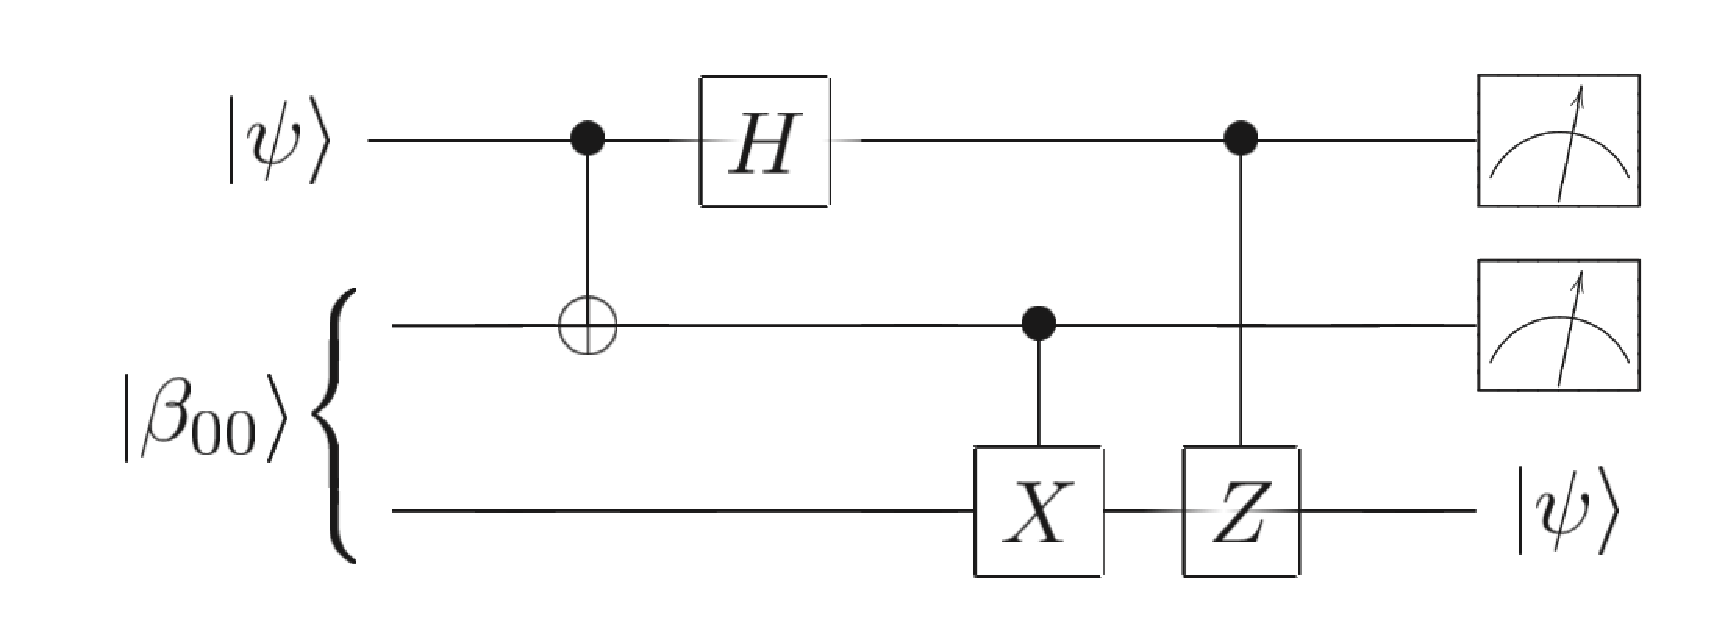
\includegraphics[width=0.5\textwidth]{circuit.pdf}
       \caption{example of a quautum circuit (taken from QCQI)}
       \label{circuit}
  \end{figure}
\end{center}

Measurement is the operation of reading information from the final state. It refers to knowing $p_{k}=\left|c_{k}\right|^{2}$ from the final state $\sum_{k=0}^{2^{n}-1} c_{k}|k\rangle$, repeating the execution and measurement of the circuit, and recording the number of times $0,1, \ldots, 2^{n_{-} 1}$ is obtained. Estimate $\left\{p_{k}\right\}$ from the histogram.





\section{Main Result}

Here is the specific algorithm.
\begin{enumerate}
  \item Convert the matrix $A$ to $e^{iAt}$ \cite{Berry2007}.
  \item Prepare the state $\ket{b}$ corresponding to $\vec{b}$ by \cite{Grover2002}.
  \item By \cite{Grover2002}, similarly prepares the state $\displaystyle \left|\Psi_{0}\right\rangle:=\sqrt{\frac{2}{T}}\sum_{\tau=0}^{T-1}\sin \frac{\pi\left(\tau+\frac{1}{2}\right)}{T}|\tau\rangle$.
  \item $\displaystyle \sum_{\tau=0}^{T-1}|\tau\rangle\langle\tau| \otimes e^{i A \tau t_{0} / T}$ (unitary) on $\left|\Psi_{0}\right\rangle \otimes|b\rangle$, where $t_{0}=O(\kappa / \epsilon)$. The tensor products of the states $\ket{b}$ and $\left|\Psi_{0}\right\rangle$ are subject to conditional Hamiltonian evolution.
\item  Perform a Fourier Transformation on the first register (register with initial state $\left|\Psi_{0}\right\rangle$).
  \item Add the qubit and make the rotation depend on the value of $\tilde{\lambda}_{k}$.
  \item Inverse Fourier Transformation.
  \item Do the inverse transform of 4.
  \item Measure the last qubit; a 1 means success and a 0 means failure.
\end{enumerate}
With the above algorithm, when the state $\ket{b}$ corresponding to the quantity $\vec{x}$ can be prepared, the computation step to find the remaining $\vec{x}^\dagger M\vec{x}$.



\section{Discussion}


\subsection{QFT}
QFT(Quantum Fourier transformation) is a operation which convert $\ket{j}$;
$$
\begin{aligned}
|j\rangle & \rightarrow \frac{1}{2^{n / 2}} \sum_{k=0}^{2^{n}-1} e^{2 \pi i j k / 2^{n}}|k\rangle \\
&=\frac{1}{2^{n / 2}} \sum_{k_{1}=0}^{1} \cdots \sum_{k_{n}=0}^{1} e^{2 \pi i j\left(\sum_{l=1}^{n} k_{l} 2^{-l}\right)}\left|k_{1} \ldots k_{n}\right\rangle \\
&=\frac{1}{2^{n / 2}} \sum_{k_{1}=0}^{1} \cdots \sum_{k_{n}=0}^{1} \bigotimes_{l=1}^{n} e^{2 \pi i j k_{l} 2^{-l}}\left|k_{l}\right\rangle \\
&=\frac{1}{2^{n / 2}} \bigotimes_{l=1}^{n}\left[\sum_{k_{l}=0}^{1} e^{2 \pi i j k_{l} 2^{-l}}\left|k_{l}\right\rangle\right] \\
&=\frac{1}{2^{n / 2}} \bigotimes_{l=1}^{n}\left[|0\rangle+e^{2 \pi i j 2^{-l}}|1\rangle\right] \\
&=\frac{\left(|0\rangle+e^{2 \pi i 0 . j_{n}}|1\rangle\right)\left(|0\rangle+e^{2 \pi i 0 . j_{n-1} j_{n}}|1\rangle\right) \cdots\left(|0\rangle+e^{2 \pi i 0 . j_{1} j_{2} \cdots j_{n}}|1\rangle\right)}{2^{n / 2}} .
\end{aligned}
$$
% The product representation (5.4) makes it easy to derive an efficient circuit for the quantum Fourier transform. Such a circuit is shown in Figure 5.1. The gate $R_{k}$ denotes the unitary transformation
% $$
% R_{k} \equiv\left[\begin{array}{cc}
% 1 & 0 \\
% 0 & e^{2 \pi i / 2^{k}}
% \end{array}\right]
% $$
% To see that the pictured circuit computes the quantum Fourier transform, consider what happens when the state $\left|j_{1} \ldots j_{n}\right\rangle$ is input. Applying the Hadamard gate to the first bit produces the state
% $$
% \frac{1}{2^{1 / 2}}\left(|0\rangle+e^{2 \pi i 0 . j_{1}}|1\rangle\right)\left|j_{2} \ldots j_{n}\right\rangle
% $$
This operation is complemented by
\begin{center}
  \begin{figure}[H]
       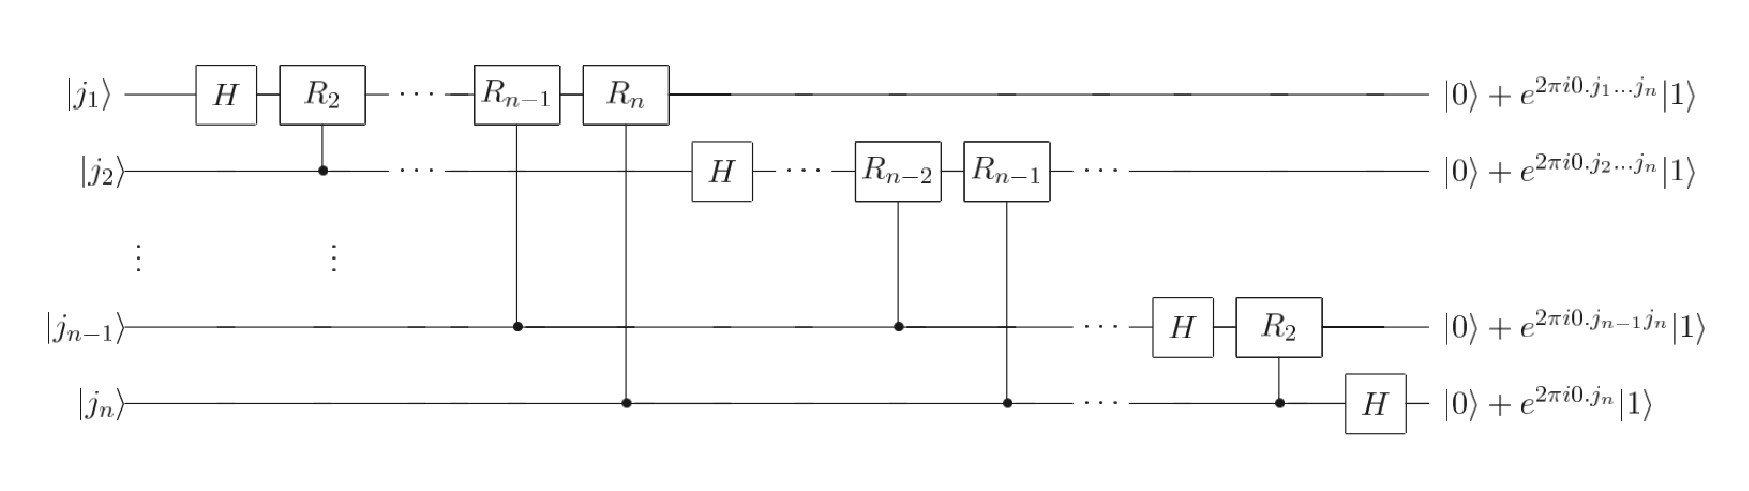
\includegraphics[width=\textwidth]{qft.pdf}
       \caption{Example of QFT(taken from QCQI)}
       \label{circuit}
  \end{figure}
\end{center}

\subsection{QPE}
QPE (Quantum Phase Estimation) is an algorithm for estimating the phase, which is calculated by applying QFT. The specific algorithm is as follows (Quoted from QCQI).
\begin{quotation}

  Inputs:

   (1) A black box wich performs a controlled- $U^{j}$ operation, for integer $j$

   (2) an eigenstate $|u\rangle$ of $U$ with eigenvalue $e^{2 \pi i \varphi_{u}}$

   (3) $t=n+\left\lceil\log \left(2+\frac{1}{2 \epsilon}\right)\right\rceil$ qubits initialized to $|0\rangle$.


  Outputs: An $n$-bit approximation $\widetilde{\varphi_{u}}$ to $\varphi_{u} .$


  Runtime: $O\left(t^{2}\right)$ operations and one call to controlled- $U^{j}$ black box. Succeeds with probability at least $1-\epsilon$.


  Procedure:


  1. $|0\rangle|u\rangle$


  2. $\quad \rightarrow \frac{1}{\sqrt{2^{t}}} \sum_{j=0}^{2^{t}-1}|j\rangle|u\rangle$ create superposition


  3. $\rightarrow \frac{1}{\sqrt{2^{t}}} \sum_{j=0}^{2^{t}-1}|j\rangle U^{j}|u\rangle$ $=\frac{1}{\sqrt{2^{t}}} \sum_{j=0}^{2^{t}-1} e^{2 \pi i j \varphi_{u}}|j\rangle|u\rangle$ apply black box


  4. $\quad \rightarrow\left|\widetilde{\varphi_{u}}\right\rangle|u\rangle$ apply inverse Fourier transform


  5. $\rightarrow \widetilde{\varphi_{u}}$ measure first register
\end{quotation}


If this is realized by a quantum circuit, it is as follows.
\begin{center}
  \begin{figure}[H]
       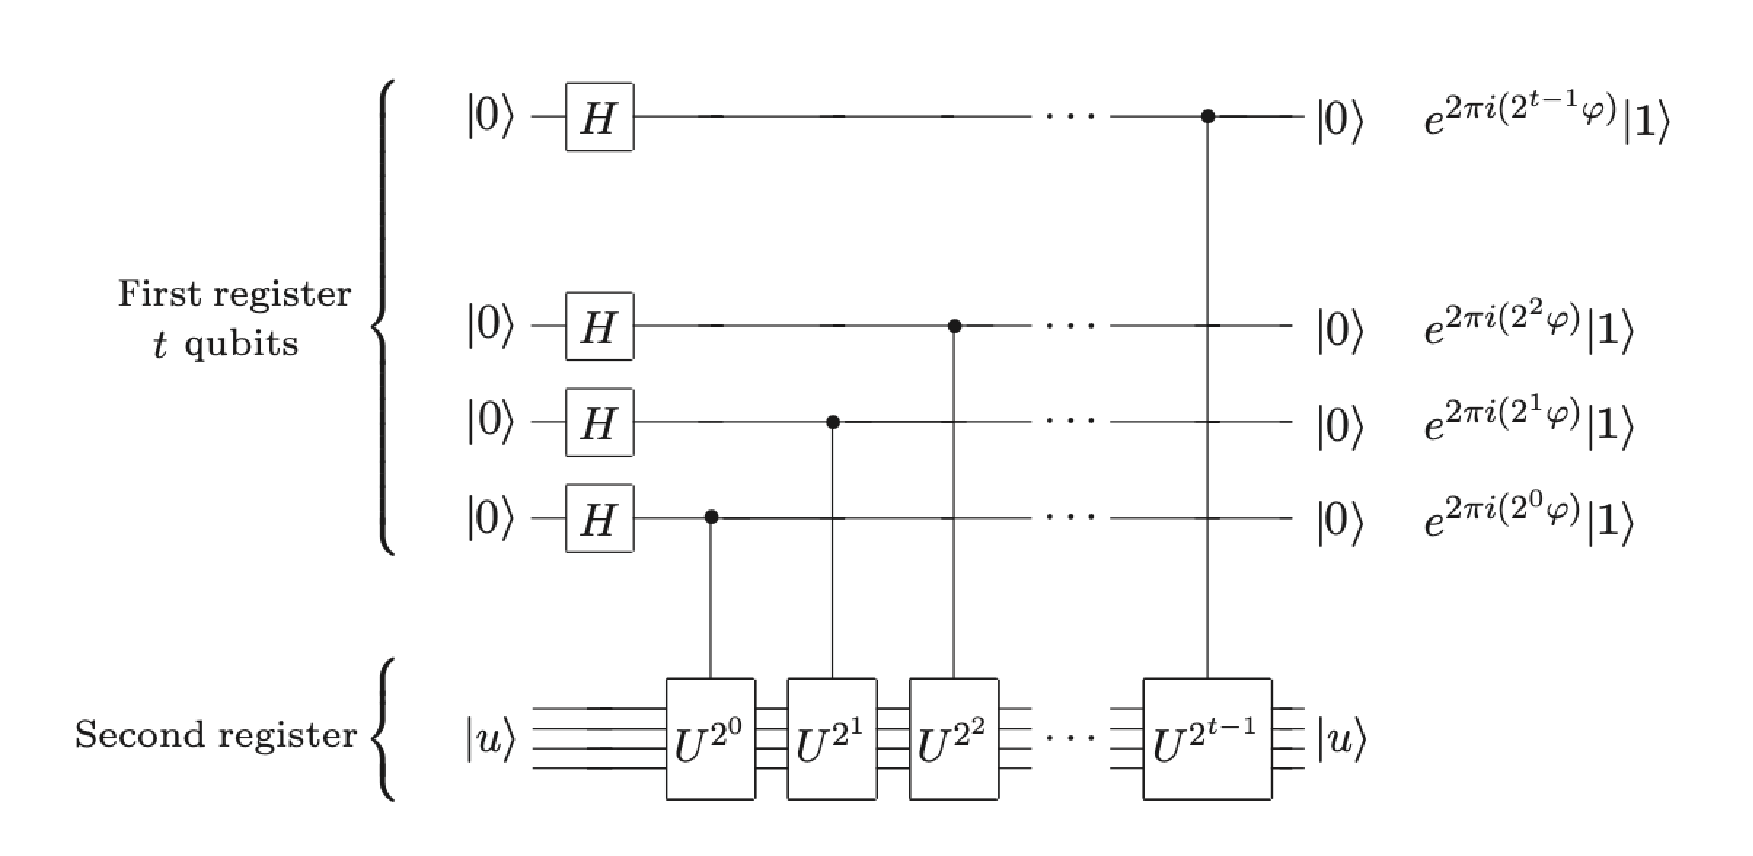
\includegraphics[width=\textwidth]{qpe.pdf}
       \caption{Examples of a part of QPE (quoted from QCQI)}
       \label{circuit}
  \end{figure}
\end{center}


\subsection{Algorithm Description}

In the following, we will explain why the algorithm introduced in the Main Result works well. First, in \cite{Berry2007}, the matrix $A$ can be computed in $\exp(iAt)$ with $O(\log(N)s^2t)$ as the upper bound.

Next, we divide the cases according to whether the matrix $A$ is Hermitian or not.

If $A$ is not Hermitian, then
\begin{eqnarray}
  \tilde{A}:= \left(\begin{array}{cc}
0 & A \\\
A^{\dagger} & 0
\end{array}\right)
\end{eqnarray}
Since $\tilde{A}$ is Hermitian by definition,
$$.
\tilde{A} \vec{y}=\left(\begin{array}{l})
\vec{b}\\\\
0
\end{array}\right)
$$.
By solving above,
$$
\vec{y}=\left(\begin{array}{l}
0 \\\
\vec{x}
\end{array}\right)
$$.
is obtained. Thus, when $A$ is not Hermitian, the series of operations to define $\tilde{A}$ and make it solvable is called reduction.

In the following, we consider the case where $A$ is Hermitian. By \cite{Grover2002}, if $b_{i}$ and $\sum_{i=i_{1}}^{i_{2}}\left|b_{i}\right|^{2}$ are efficiently computable, then state $\ket{b}$ in an arbitrary basis for arbitrary probability amplitudes. If $\ket{b}$ is efficiently computable, then state $\ket{b}$ can be converted to a superposition for any probability amplitude in any basis. We will denote $\ket{b}$ by the superposition of the eigenvectors (choose a unit vector) of $A$. For the probability amplitude, we consider assigning a component of $\vec{b}$. Now we also define $\left|u_{j}\right\rangle$ as the eigenvectors of $A$ , and $\lambda_{j}$ as the corresponding eigenvalues. So far, $\ket{b}$ is ready.

$$.
\left|\Psi_{0}\right\rangle:=\sqrt{\frac{2}{T}}\sum_{\tau=0}^{T-1}\sin \frac{\pi\left(\tau+\frac{1}{2}\right)}{T}\tau\rangle
$$.

However, here $T$ is assumed to be a very large value. This gives us $\left|\Psi_{0}\right\rangle$ is now ready. By applying conditional Hamiltonian evolution to the tensor products of $\ket{b}$ and $\left|\Psi_{0}\right\rangle$ prepared in this way

$\sum_{\tau=0}^{T-1}|\tau\rangle\langle\tau|\otimes e^{i A \tau t_{0} / T}$ (unitary) on $\left|\Psi_{0}\right\rangle\otimes|b\rangle$, where $t_{0}=O(\kappa / \epsilon)$. By Fourier Transformation of the first register (the register whose initial state is $\left|\Psi_{0}\right\rangle$), we get The state in the first register is

$$.
\sum_{j=1}^{N} \sum_{k=0}^{T-1} \alpha_{k \mid j} \beta_{j}|k\rangle\left|u_{j}\right\rangle
$$.

Replacing $\ket{k}$ with $\left|\tilde{\lambda}_{k}\right\rangle$.

$$.
\sum_{j=1}^{N} \sum_{k=0}^{T-1} \alpha_{k \mid j} \beta_{j}\left|\tilde{\lambda}_{k}\right\rangle\left|u_{j}\right\rangle
You can do that with $$.
We can add a qubit and rotate $\left|\tilde{\lambda}_{k}\right\rangle$ to get

$$.
\sum_{j=1}^{N} \sum_{k=0}^{T-1} \alpha_{k \mid j} \beta_{j}\left|\tilde{\lambda}_{k}\right\rangle\left|u_{j}\right\rangle\left(\sqrt{1-\frac{C^{2}}{\tilde{\lambda}_{k}^{2}}}|0\rangle+\frac{C}{\tilde{\lambda}_{k}}|1\rangle\right)
$$.

However, $C$ is $O(1 / \kappa)$. Phase estimation allows us to calculate $\left|\tilde{\lambda}_{k}\right\rangle $ backwards. If phase estimation is perfect, then$\alpha_{k \mid j}=1$ if $\tilde{\lambda}_{k}=\lambda_{j}$, and 0 otherwise.

Then,
$$
\sum_{j=1}^{N} \beta_{j}\left|u_{j}\right\rangle\left(\sqrt{1-\frac{C^{2}}{\lambda_{j}^{2}}}|0\rangle+\frac{C}{\lambda_{j}}|1\rangle\right)
$$
If we measure the last qubit, we get last
$$
\sqrt{\frac{1}{\sum_{j=1}^{N} C^{2}\left|\beta_{j}\right|^{2} /\left|\lambda_{j}\right|^{2}}} \sum_{j=1}^{N} \beta_{j} \frac{C}{\lambda_{j}}\left|u_{j}\right\rangle
$$
This corresponds to $|x\rangle=\sum_{j=1}^{n}\beta_{j}\lambda_{j}^{-1}\left|u_{j}\right\rangle$. If we measure with $M$, we get $\langle x|M| x\rangle$.
% Runtime and error analysis.
% Runtime and error analysis.-We present an informal description of the sources of error; the exact error analysis and runtime considerations are We present an informal description of the sources of error; the exact error analysis and runtime considerations are presented in Ref. Performing the phase estimation is done by simulating $e^{i A t}$. Assuming that $A$ is $s$ sparse, this can be done with error $\epsilon$ in time proportional to $t s^{2}(t / \epsilon)^{o(1)}=: \tilde{O}\left(t s^{2}\right)$.
%.This step errs by $O\left(1 / t_{0}\right)$ in estimating $\lambda$, which translates into a relative error of $O\left(1 / t_{0}\right)$. This step errs by $O\left(1 / \lambda t_{0}\right)$ in estimating $\lambda$, which translates into a relative error of $O\left(1 / \lambda t_{0}\right)$ in $\lambda^{-1}$. If $\lambda \geq 1 / \kappa$, taking $t_{0}=O(\kappa / \epsilon)$ induces a final error of $\epsilon$. Finally, we consider the success probability of the post-selection process. Since $C=O(1 / \kappa)$ and $\lambda \leq 1$, this probability is at least Since $C=O(1 / \kappa)$ and $\lambda \leq 1$, this probability is at least $\Omega\left(1 / \kappa^{2}\right)$. Using amplitude amplification [14], we find


\section{Conclusion}
Solving the linear system of equations $A\vec{x}=\vec{b}$ is an important problem in any field\cite{Harrow2009}, and it is not necessary to know $\vec{x}$ itself, but if we want to find a quantity related to $\vec{x}$, such as $\vec{x}^\dagger M$, we can apply quantum phase estimation to find it probabilistically. The success probability depends on the condition number $\kappa $.
% \begin{enumerate}
%\item Prepare the states $\ket{b}$, $\left|\Psi_{0}\right\rangle$.
%\item Convert the matrix $A$ to $e^{iAt}$ and set $\displaystyle \sum_{\tau=0}^{T-1}|\tau\rangle\langle\tau|\otimes e^{i A \tau t_{0} / T}$ (unitary) on $\left|\Psi_{0}\right\rangle \otimes|b\rangle$, where $t_{0}=O(\kappa / \epsilon)$.
% Fourier Transformation of \item first register (register with initial state $\left|\Psi_{0}\right\rangle$).
% Add the \item qubit and rotate it.
%\item phase estimation.
% Measure the \item last qubit.
%\end{enumerate}
When the state $\ket{b}$ corresponding to $\vec{b}$ is ready, the computational step to find $\ket{x}$ can be computed on a polynomial time scale of $\log(N), \kappa $. This is an exponential speedup compared to the fastest known algorithm on a classical computer.

% \section{Appendix}
% No plans to include

\section{Reference}


%\cite{Reference Name}
% Neubig et al. \cite{KyTea}
%\bibliographystyle{osajnl}
%\bibliographystyle{plain}
%\bibliography{test}

\bibliography{ref} %hoge.bibから拡張子を外した名前
\bibliographystyle{unsrt} %参考文献出力スタイル





\end{document}
